% ===================================================================
% Arquivo: capitulos/parte-III-pilares/cap-10-perda-binaria.tex
% ===================================================================

\chapter{Funções de Perda para Regressão}
\label{cap:perda-regressao}

Até agora foi visto o funcionamento da retropropagação, e como ela faz uso dos otimizadores, os quais funcionam como um barco, percorrendo a função de perda em busca de pontos de mínimos. Além disso, em seguida foram vistas diversas funções de ativação, começando pelas sigmoidais, depois pelas retificadoras, e por fim uma coletânea de diferentes funções. Contudo, está na hora de entender o outro lado da retropropagação: as funções de perda.

Para isso, esse capítulo busca explicar diversas funções de perda e suas aplicações, começando pelas funções para problemas de regressão, conhecendo as clássicas erro quadrático médio e erro absoluto médio, além da \textit{hubber loss}, uma função que busca unir o melhor dessas duas funções de perda. Seguindo adiante, são introduzidas as funções de perda para classificação binária, como a \textit{BCE}. Visto os problemas de classificação binária, é possível também conhecer os problemas de classifação multi com a \textit{categorical cross entropy}.

Mais adiante, está apresentado não funções, mas esquemas de como a perda pode ser medida para problemas como o de redes adversárias. Mas as perdas não são a única forma de medir como um modelo está performando, para isso, o final do capítulo é dedicado para explicar outros diferentes métodos de medir o desempenho do modelo que está sendo construído.

\section{A Intuição da Perda: Medindo o Erro do Modelo}

\section{Exemplo Ilustrativo: Jogando Dados}

Pense que você está jogando dardos com seus amigos e quer decidir quem está com mais pontos. Mas você não está satisfeito em considerar as marcações que estão no jogo, e decidiu inovar. Para isso, você pegou uma régua e passou a medir a distância que os dardos que você e seus amigos haviam jogado no centro. Quem chegasse mais próximo do centro, ganhava o jogo.

Essa ideia de medir o quão próximo você está do resultado desejado utilizando a disância entre esses dois pontos como parâmetro, é justamente o motivador pela criação das funções de perda para regressão. Para isso, elas utilizam diferentes fórmulas, com todas com o mesmo intuito, medir a distância em que o "chute" dado pelo modelo está do ponto real (desejado).

\section{Funções de Perda para Regressão para Propósitos Gerais}

\subsection{Erro Quadrático Médio (Mean Squared Error - MSE)}

A primeira função de perda a ser vista nesse capítulo é a erro quadrático médio (\textit{mean squared error}) também conhecida com \textit{MSE}. Suas origens são voltadas para o século XIX, com o avanço dos estudos da astronomica, em que os estudiosos buscavam entender o comportamento das estrelas e dos outros planetas. A \textit{MSE} surge naturalmente no trabalho \textit{Nouvelles méthodes pour la détermination des orbites des comètes} (Novos métodos para determinar as órbitas dos cometas), nele \textcite{Legendre1805} introduz o método conhecido como método dos mínimos quadrados, o qual tem como objetivo minimizar a soma dos quadrados dos erros.

Contudo, o trabalho de Legendre não foi o único resposável por popularizar o método dos mínimos quadrados. Em \textit{Theoria Motus Corporum Coelestium in Sectionibus Conicis Solem Ambientium}, \textcite{Gauss1809}, em uma série de artigos, discute um problema que se inicia com um sistema de equações linerares com mais equações que icognitas derivadas de observações atronômicas que possuem erros, seu objetivo é então encontrar o valor mais provável para essas icôgnitas.

Para isso, Gauss define que o valor mais provável de uma quantidade de medidas de igual precisão é dado pela média aritmética dessas medidas \parencite{Gauss1809}. Com base nisso, \textcite{Gauss1809} se pergunta qual deve ser a lei de probabilidade dos erros para que a média aritmética seja sempre a estimativa mais provável, para resolver esse problema ele utiliza o princípio da máxima-verossimilhança das probabilidades de todos os erros, e com ele, Gauss consegue ser capaz de demonstrar matematicamente que a única função que satisfaz o seu postulado da média aritmética é a própria distribuição Normal.

Sabendo disso, Gauss inverte a lógica: se a probabilidade de um conjunto de erros é máximizada quando a soma dos seus quadrados é minimizada, então o método dos mínimos quadrados é o método que dá a solução mais provável para a suposição de que os erros de medição são normalmente distribuídos \parencite{Gauss1809}. Dessa forma, o matemático foi capaz de adicionar mais embasamento matemático na técnica de Legedre, e com isso aumentando a popularização do \textit{MSE}.

Passado quase 200 anos, o erro quadrático médio se torna uma das principais funções a ser utilizada para calcular o erro dos modelos. Caso você tenha lido o Capítulo \ref{cap:retropropagacao-gradiente}, pode ter notado que ela foi uma das funções, junto com a sigmoide logística e a equação do neurônio, a ser utilizada para deduzir os cálculos das atualizações de pesos para o algoritmo da retropropagação \parencite{BackpropagationArticle}.

Assim, é possível agora apresentar a fórmula do \textit{MSE}, o qual é calculado através da Equação \ref{eq:mse}.

\begin{equacaodestaque}{Erro Quadrático Médio (MSE)}
    \Loss_{\text{MSE}} = \frac{1}{N} \sum_{j=1}^{N} (y_j - \hat{y}_j)^2
    \label{eq:mse}
\end{equacaodestaque}

Em que:

\begin{itemize}
    \item $y_j$ representa o valor previsto para a saída;
    \item $\hat{y}_j$ representa o valor predito pelo modelo;
    \item $N$ representa o número de predições feitas.
\end{itemize}

Neste caso, o \textit{MSE} calcula o erro individualmente para cada uma das predições, soma esses valores e em seguida calcula a média.

Tendo a sua equação, é possível também plotar o seu gráfico, para isso, ele pode ser visto na Figura \ref{fig:mse}.

\begin{figure}
    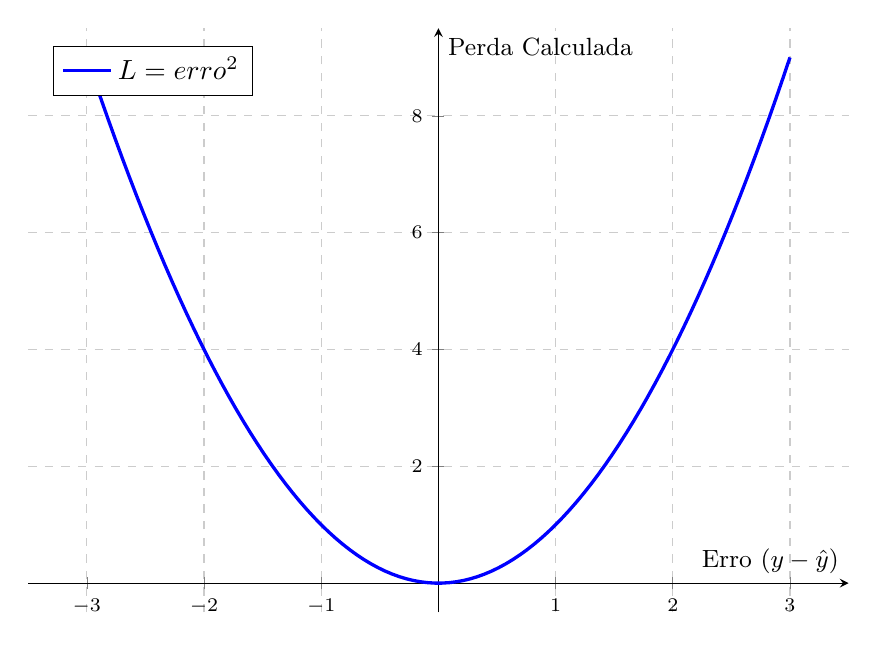
\begin{tikzpicture}
        \begin{axis}[
            xlabel={Erro ($y - \hat{y}$)},
            ylabel={Perda Calculada},
            axis lines=middle,          % Eixos centrados em (0,0)
            grid=major,                 % Adiciona uma grade principal
            grid style={dashed, gray!40}, % Estilo da grade
            xmin=-3.5, xmax=3.5,        % Limites do eixo x
            ymin=-0.5, ymax=9.5,         % Limites do eixo y
            legend pos=north west,      % Posição da legenda
            width=12cm,                 % Largura do gráfico
            height=9cm,                 % Altura do gráfico
            title style={font=\bfseries},
            label style={font=\small},
            tick label style={font=\scriptsize}
        ]
            % Adiciona o gráfico da função x^2
            \addplot[
                domain=-3:3, 
                samples=100, 
                color=blue, 
                very thick
            ] {x^2};
            
            % Adiciona uma entrada na legenda
            \addlegendentry{$L = \text{erro}^2$}
        \end{axis}
    \end{tikzpicture}
    \caption{Função de perda para regressão erro quadrático médio (\textit{MSE}).}
    \label{fig:mse}
    \fonte{O autor (2025).}
\end{figure}

Tendo o seu gráfico e sua equação é possível discutir algumas propriedades interessantes do erro quadrático médio, entre elas vale destacar:

\begin{itemize}
    \item \textbf{Não-negatividade:} Como é visto no gráfico da Figura \ref{fig:mse}, o \textit{MSE} é uma função que retorna apenas valores positivos, isso se dá devido a diferença das entradas estar sendo calculada e logo em seguida elavada ao quadrado, impendido que valores negativos ocorram na saída.
    \item \textbf{Sensibilidade para \textit{outliers}}: Como \textcite{LossesArticle} discutem, a função erro quadrático médio possui a tendência de punir em maior força os erros que são originarios de uma distância muito grande. Isso acontece por conta do jeito que é calculada essa função, lembre que ela calcula a distância entre os pontos e depois eleva ela ao quadrado, se essa distância for muito grande, o erro será maior ainda. Como consequência, se existe um conjunto grande de pontos que ficam fora da regressão, os \textit{outliers}, a função de perda irá constamente retornar valores altos. Isso pode atrapalhar o aprendizado, porque será mais difícil otimizar o modelo, mas também pode ser uma vantagem em cenários em que os erros devem ser fortemente penalizados.
    \item \textbf{Convexa (nas predições):}: Voltando para a Figura \ref{fig:mse} é possível notar que o \textit{MSE} é uma função convexa, o seu gráfico tem a típica forma de um funíl, apresentando um único ponto de mínimo global, isso ajuda na otimização dessa função caso se esteja usando um otimizador baseado no gradiente descendente. Contudo, \textcite{LossesArticle} destacam que em redes neurais profundas essa função pode se tornar não-convexa, devido as transformações não-lineares que são feitas ao construir o modelo.
    \item \textbf{Baixa intepretabilidade:} Note que a função \textit{MSE} eleva o erro ao quadrado, de forma que ao mostrar a perda não é visto diretamente a distância entre os pontos reais e os pontos preditos pelo modelo. Isso um gera um gargalo pois não é possível de forma instânea saber exatamente quão bem ou mal o modelo está performando. Funções como a \textit{MAE}, em que o erro é calculado como o módulo da distância entre os dois pontos são mais diretas em mostrar a performance do modelo.
    \item \textbf{Continuidade:} Ainda na Figura \ref{fig:mse} é possível notar que o \textit{MSE} é uma função contínua em todo o seu domínimo, isso é uma vantagem muito boa, pois indica que é possível derivar essa função sem encontrar grandes problemas.
\end{itemize}

Além disso, cabe também destacar a derivada da função \textit{MSE}, a qual está presente na Equação \ref{eq:mse-derivada}. A derivada de uma função de perda é de extrema utilizada para uma rede neural, pois é a partir dela que é calculado o primeiro vetor gradiente, este, é calculado com base na derivada da função de perda para a saída da rede, e passa então a ser retropropagado por toda a rede no sentido inverso, indo primeiro das últimas camadas para as camadas de entrada.

Note que diferente das funções de ativação em que era calculada a sua derivada ordinária, aqui é calculado as derivadas parciais das funções de perda para cada um dos seus componentes, a saída do modelo $\hat{y}_j$ e a saída esperada $y_j$. Com base nessas duas derivadas, é possível construir o vetor gradiente.

\begin{equacaodestaque}{Erro Quadrático Médio (\textit{MSE}) Derivada}
    \frac{\partial \Loss_{\text{MSE}}}{\partial \hat{y}_j} = \frac{2}{N}(\hat{y}_j - y_j)
    \label{eq:mse-derivada}
\end{equacaodestaque}

Tendo a sua derivada, vale a pena analisar também o seu gráfico, para isso, é possível vê-lo na Figura \ref{fig:mse-derivada}. 

\begin{figure}[h!]
    \centering
    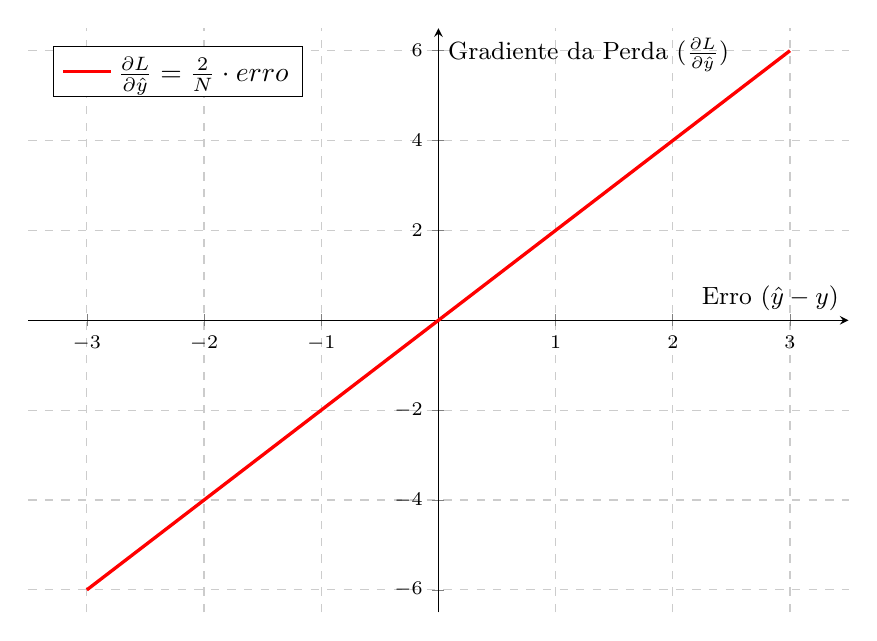
\begin{tikzpicture}
        \begin{axis}[
            xlabel={Erro ($\hat{y} - y$)},
            ylabel={Gradiente da Perda ($\frac{\partial L}{\partial \hat{y}}$)},
            axis lines=middle,
            grid=major,
            grid style={dashed, gray!40},
            xmin=-3.5, xmax=3.5,
            ymin=-6.5, ymax=6.5,
            legend pos=north west,
            width=12cm,
            height=9cm,
            title style={font=\bfseries},
            label style={font=\small},
            tick label style={font=\scriptsize}
        ]
            % Adiciona o gráfico da função 2*x
            \addplot[
                domain=-3:3, 
                samples=100, 
                color=red, 
                very thick
            ] {2*x};
            
            % Adiciona uma entrada na legenda
            \addlegendentry{$\frac{\partial L}{\partial \hat{y}} = \frac{2}{N} \cdot \text{erro}$}
        \end{axis}
    \end{tikzpicture}
    \caption{Gráfico da derivada da função de perda erro quadrático médio (\textit{MSE}).}
    \label{fig:mse-derivada}
    \fonte{O autor (2025).}
\end{figure}

É possível perceber pelo gráfico da derivada da função de perda erro quadrático médio que o gradiente da perda é proporcional ao erro. Seguindo essa lógica, se o erro está alto, o gradiente também estará alto, como consequência as atualizações de pesos e vieses, as quais seguem o método do gradiente (visto nas Equações ) serão mais bruscas, dando maiores saltos no gráfico da função de perda. Enquanto em situações que o erro está pequeno em magnitudade, o gradiente também será pequeno e o modelo fará pequenas atualizações nos seus parâmetros, garantindo um ajuste fino.

\begin{equation}
    \frac{\partial E}{\partial w_{ji}} = \frac{\partial E}{\partial x_j} \cdot y_i \quad \text{ou} \quad \frac{\partial E}{\partial w_{ji}} = \frac{\partial E}{\partial y_j} \cdot \sigma'(x_j) \cdot y_i
    \label{eq:gradiente-do-erro-em-relacao-a-um-peso-de-um-neuronio-perda-regressao}
\end{equation}

Conhecendo a função de perda \textit{MSE}, é possível agora discutir uma outra abordagem para resolver problemas de regressão. Para isso, a próxima seção busca apresentar o erro absoluto médio, que é uma alternativa para o erro quadrático médio que tem como principal diferença o jeito que lida com \textit{outliers}.

\subsection{Erro Absoluto Médio (Mean Absolute Error - MAE)}

O erro absoluto médio é uma função que tem o mesmo propósito do erro quadrático médio, ser utilizada para tarefas de regressão. Neste caso o \textit{MAE} não possui uma origem definida que como o \textit{MSE}, esse conceito de minimizar a diferença de um resultado pelo seu valor real já havia sendo utilizado a bastante tempo. Contudo, trabalhos como \textit{Greedy function approximation: A gradient boosting machine} de \textcite{GreedyFunctionApproximation} fazem uso do erro absoluto médio para resolver problemas de aprendizado de máquina. No texto, o autor desenvolve um algoritmo de \textit{boosting} específico para o \textit{MAE}, neste caso, ela é apresentada com outro nome, \textit{Least-Absolute-Deviation} (\textit{LAD}), sendo responsável por dar nome ao algoritmo criado, o \texttt{LAD\_TreeBoost} \parencite{GreedyFunctionApproximation}. Neste caso, \textcite{GreedyFunctionApproximation} explica que esse algoritmo faz uso de uma árvore de regressão com a perda, de forma que para prever a pseudo-resposta que é o sinal dos resíduos atuais é utilizado o método dos mínimos quadrados. Assim, o modelo é atualizado adicionando em cada nó terminal da nova árvore criada a mediana dos resíduos daquela região específica.

Um trabalho mais recente que explora o uso dessa função é o \textit{Image-to-Image Translation with Conditional Adversarial Networks} \parencite{ImageToImage}. Nele, \textcite{ImageToImage} argumentam que preferiram trabalhar com a função de perda \textit{L1 distance} (um dos diferentes nomes utilizados para se referir ao \textit{MAE}) devido a essa função gerar imagens menos borradas. É possível ver essa comparação nas imagens da Figura \ref{fig:comparativo-perdas-image-to-image}. Perceba que a perda que apresenta os resultados mais consistentes com a realidade é justamente a \textit{L1 + cGAN}, a qual possuí o \textit{MAE} em sua composição.

\begin{figure}[h]
    \centering
    \includegraphics[width=0.65\linewidth]{../imagens/perda-regressao/image-to-image-perdas-comparativo.png}
    
    \caption[CurvPerdas diferentes induzem qualidades de resultados diferentes. Cada coluna mostra resultados treinados sob uma perda diferenteas de aprendizado no dataset MNIST]{%
        \newline
        \small Fonte: \parencite{ImageToImage}.
    }
    \label{fig:comparativo-perdas-image-to-image}
\end{figure}

Visto esses diferentes cenários em que o erro absoluto médio foi utilizado para resolver problemas de regressão é possível ver agora a sua definição matemática, para isso, o \textit{MAE} está definido na Equação \ref{eq:mae}. Perceba que ele é responsável por calcular a diferença entre os dois pontos, o valor real $\hat{y}_j$ e o valor predito $y_j$, para todos os $N$ casos analisados e a partir disso calcular a média dos resultados.

\begin{equacaodestaque}{Erro Absoluto Médio (\textit{MAE})}
    \Loss_{\text{MAE}} = \frac{1}{N} \sum_{j=1}^{N} |y_j - \hat{y}_j|
    \label{eq:mae}
\end{equacaodestaque}

Também vale a pena analisar o \textit{MAE} de forma gráfica, para isso ele está representado na Figura \ref{fig:mae}.

\begin{figure}
    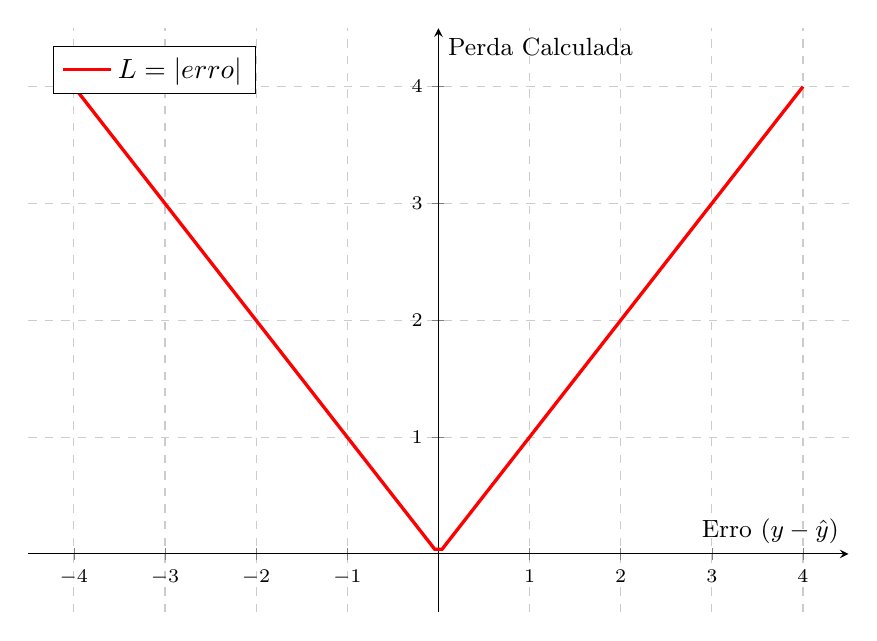
\begin{tikzpicture}
        \begin{axis}[
            xlabel={Erro ($y - \hat{y}$)},
            ylabel={Perda Calculada},
            axis lines=middle,          % Eixos centrados em (0,0)
            grid=major,                 % Adiciona uma grade principal
            grid style={dashed, gray!40}, % Estilo da grade
            xmin=-4.5, xmax=4.5,        % Limites do eixo x
            ymin=-0.5, ymax=4.5,         % Limites do eixo y
            legend pos=north west,      % Posição da legenda
            width=12cm,                 % Largura do gráfico
            height=9cm,                 % Altura do gráfico
            title style={font=\bfseries},
            label style={font=\small},
            tick label style={font=\scriptsize}
        ]
            % Adiciona o gráfico da função abs(x)
            \addplot[
                domain=-4:4, 
                samples=100, 
                color=red, 
                very thick
            ] {abs(x)};
            
            % Adiciona uma entrada na legenda
            \addlegendentry{$L = |\text{erro}|$}
        \end{axis}
    \end{tikzpicture}
    \caption{Gráfico da função de perda erro absoluto médio (\textit{MAE}).}
    \label{fig:mae}
    \fonte{O autor (2025).}
\end{figure}

A partir do seu gráfico e de sua equação é possível retirar diferentes informações dessa função de perda, as quais estão discutidas a seguir:

\begin{itemize}
    \item \textbf{Não-negatividade:} Como é possível ver em seu gráfico da Figura \ref{fig:mae}, o erro absoluto médio compartilha dessa mesma propriedade com o \textit{MSE}, isso significa que sua saída será sempre positiva ou zero, independente do valor de entrada. Isso se dá, devido a propriedade do módulo, que não admite números negativos para sua saída.
    \item \textbf{Robustez para \textit{outliers}}: Como \textcite{LossesArticle} explicam, o \textit{MAE} não penaliza os \textit{outliers} de forma tão severa como o erro quadrático médio. Isso acontece pois diferente do \textit{MSE}, em que o erro cresce de forma quadrática, no \textit{MAE}, ele cresce de forma linear, significando que diferente do \textit{MSE} que era sensível aos \textit{outliers}, o \textit{MAE} também reage à eles, mas de forma menos severa.
    \item \textbf{Convexa (nas predições):} Voltando para o seu gráfico, é possível ver que o erro absoluto médio segue a mesma forma de funíl do erro quadrático médio, podendo ser considerado uma função convexa e com um só ponto de mínimo global. Contudo, assim como no \textit{MSE}, \textcite{LossesArticle} advertem que para modelos de apredenziado profundo, o \textit{MAE} pode deixar de ser uma função convexa devido às muitas camadas e funções não-lineares.
    \item \textbf{Não-derivável em zero:} Esse ponto acontece justamente devido a forma que a função apresenta, ela faz uma especíe de "bico" em zero, além disso, ao calcular os seus limites laterais para verificar a continuidade da função é possível notar que eles apresentam valores diferentes.
\end{itemize}

Se a função não é derivável em zero, é esperado que ela não seja uma boa alternativa para ser utilizada junto com otimizadores baseados na descida do gradiente, pois, pontos de descontinuidade como esse podem acabar atrapalhando a forma com que o modelo é otimizado. Contudo, \textcite{LossesArticle} argumentam, é possível resolver esse problema utilizado técnicas de subgradiente, sendo possível então escrever a derivada do \textit{MAE} com a Equação \ref{eq:mae-derivada}.

\begin{equacaodestaque}{Erro Absoluto Médio (\textit{MAE}) Derivada}
    \frac{\partial \Loss_{\text{MAE}}}{\partial \hat{y}_j} = 
    \begin{cases} 
      -1 & \text{se } \hat{y}_j > y_j \\
      +1 & \text{se } \hat{y}_j < y_j \\
      [-1, +1] & \text{se } \hat{y}_j = y_j
    \end{cases}
    \label{eq:mae-derivada}
\end{equacaodestaque}

Contudo, mesmo possuindo esse detalhe de descontinuidade em zero, isso não atrapalha a plotagem do gráfico do \textit{MAE}, o qual está representado na Figura \ref{fig:mae-derivada}.

\begin{figure}[h!]
    \centering
    \begin{tikzpicture}
        \begin{axis}[
            xlabel={Erro ($\hat{y} - y$)},
            ylabel={Gradiente da Perda ($\frac{\partial L}{\partial \hat{y}}$)},
            axis lines=middle,
            grid=major,
            grid style={dashed, gray!40},
            xmin=-3.5, xmax=3.5,
            ymin=-1.5, ymax=1.5,
            ytick={-1, 0, 1}, % Define os pontos no eixo y
            legend pos=north west,
            width=12cm,
            height=9cm,
            title style={font=\bfseries},
            label style={font=\small},
            tick label style={font=\scriptsize}
        ]
            % Parte negativa da derivada (-1)
            \addplot[
                domain=-3:0, 
                samples=100, 
                color=red, 
                very thick
            ] {-1};

            % Parte positiva da derivada (+1)
            \addplot[
                domain=0:3, 
                samples=100, 
                color=red, 
                very thick
            ] {1};
            
            % Adiciona círculos abertos para indicar a descontinuidade em x=0
            \addplot[only marks, mark=o, color=red, mark size=2pt] coordinates {(0,-1) (0,1)};
        \end{axis}
    \end{tikzpicture}
    \caption{Gráfico da derivada da função de perda erro absoluto médio (\textit{MAE}).}
    \label{fig:mae-derivada}
    \fonte{O autor (2025).}
\end{figure}

Perceba que a derivada do erro absoluto médio é representado em forma de uma função por partes, neste caso, ela é divida em duas diferentes retas, parecida com a função de ativação degrau unitário. Assim, a derivada do \textit{MAE} é composta por duas retas constantes, a primeira constante em $-1$ e a segunda constante em $1$, apresentando uma descontinuidade em zero.

Visto o erro quadrático médio, que penaliza fortamente ou \textit{outliers}, e o erro absoluto médio, que não penaliza de forma agressiva os \textit{outliers}, surge uma pergunta: Existe alguma forma de ter uma função que penalize os erros gravemente até um certo ponto e depois desse, ela não se preocupe tanto com os \textit{outliers}? Essa é a proposta da perda Huber, a qual busca unir os principais benefícios dessas duas funções de regressão. Ela será vista em seguida.

\subsection{Huber Loss: O Melhor de Dois Mundos}

A Huber \textit{Loss} recebe o seu nome devido ao seu criador, Peter J. Huber, que apresentou para a comunidade científica no trabalho \textit{Robust Estimation of a Location Parameter} \parencite{HuberLoss}. No artigo, \textcite{HuberLoss} define um estimador robusto $p$ que segue a Equação \ref{eq:huber-loss-do-huber}.

\begin{equation}
    p(t) = 
    \begin{cases}
        \frac{1}{2} t^2 \text{para} |t| < k \\
        k |t| - \frac{1}{2} k^2 para t \ge k
    \end{cases}
    \label{eq:huber-loss-do-huber}
\end{equation}

O que Huber estava querendo basicamente era uma função que se comportasse de forma quadrática para os casos em que $|t| < k$ e que se comportasse de forma linear para os casos em que $t \ge k$. Essa função criada pelo pesquisador é a função que está sendo estudada, a perda Huber, a qual pode ser representada, agora com notações voltadas para o cenário de aprendizado de máquina, com a Equação \ref{eq:huber-loss}.

\begin{equacaodestaque}{Huber Loss}
    \Loss_{\text{Huber}}(y, \hat{y}) = 
    \begin{cases} 
      \frac{1}{2}(y - \hat{y})^2 & \text{para } |y - \hat{y}| \le \delta \\
      \delta (|y - \hat{y}| - \frac{1}{2}\delta) & \text{caso contrário}
    \end{cases}
    \label{eq:huber-loss}
\end{equacaodestaque}

É possível também representar a perda Huber utilizando gráficos, para isso, ela pode ser vista na Figura \ref{fig:huber-loss}. Perceba que é como se ela fosse duas funções em uma, até um certo ponto do gráfico ela age parecido a uma função quadrática, contudo, após passar do limite de $\delta$ ela passa a ser uma função linear.

\begin{figure}
    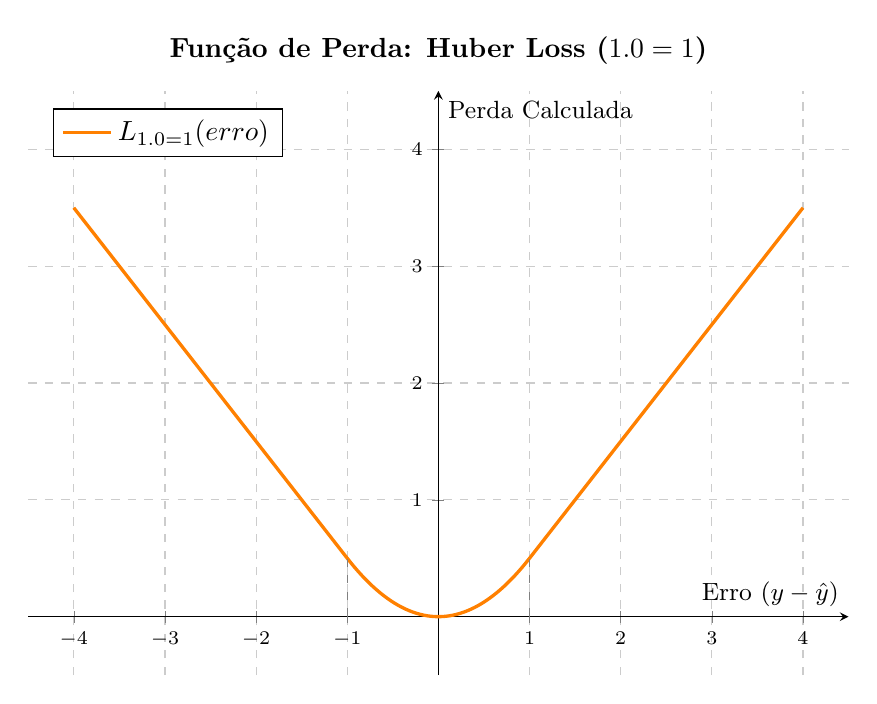
\begin{tikzpicture}
        \begin{axis}[
            title={Função de Perda: Huber Loss ($\delta=1$)},
            xlabel={Erro ($y - \hat{y}$)},
            ylabel={Perda Calculada},
            axis lines=middle,          % Eixos centrados em (0,0)
            grid=major,                 % Adiciona uma grade principal
            grid style={dashed, gray!40}, % Estilo da grade
            xmin=-4.5, xmax=4.5,        % Limites do eixo x
            ymin=-0.5, ymax=4.5,         % Limites do eixo y
            legend pos=north west,      % Posição da legenda
            width=12cm,                 % Largura do gráfico
            height=9cm,                 % Altura do gráfico
            title style={font=\bfseries},
            label style={font=\small},
            tick label style={font=\scriptsize}
        ]
            % Define o valor de delta
            \def\delta{1.0}

            % Adiciona o gráfico da função Huber usando uma expressão condicional
            % Se |x| <= delta, usa 0.5*x^2. Senão, usa delta*(|x| - 0.5*delta).
            \addplot[
                domain=-4:4, 
                samples=201, % Samples ímpares para incluir o ponto x=0
                color=orange, 
                very thick
            ] { abs(x) <= \delta ? 0.5*x^2 : \delta*(abs(x) - 0.5*\delta) };
            
            % Adiciona uma entrada na legenda
            \addlegendentry{$L_{\delta=1}(\text{erro})$}

            % Opcional: Adiciona linhas para mostrar a transição em delta
            \draw[dashed, gray] (axis cs:-\delta, 0) -- (axis cs:-\delta, {\delta*(\delta-0.5*\delta)});
            \draw[dashed, gray] (axis cs:\delta, 0) -- (axis cs:\delta, {\delta*(\delta-0.5*\delta)});

        \end{axis}
    \end{tikzpicture}
    \caption{Gráfico da função de perda erro Huber \textit{loss}.}
    \label{fig:huber-loss}
    \fonte{O autor (2025).}
\end{figure}

Conhecido o gráfico e sua equação, é possível agora discutir algumas das propriedades da perda huber, as quais são apresentadas a seguir:

\begin{itemize}
    \item \textbf{Robustez para \textit{outliers}:} Assim como o \textit{MAE}, a perda Huber não penaliza de forma quadrática os erros como comparado com o erro quadrático médio, dessa forma, os \textit{outliers} não conseguem afetar desticmaente o cálculo da perda dependendo do valor de $\delta$ escolhido \parencite{LossesArticle}.
    \item \textbf{Diferenciabilidade em $\delta$:} Um ponto a ser destacado ao se utilizar a perda Huber é que ela apresenta pontos de descontinuidade para o cenário em que $y - \hat{y} = \delta$, contudo a função é contínua em todo o resto, dessa forma, isso não a impede de ser utilizada em conjunto com otimizadores baseados em gradiente \parencite{LossesArticle}.
\end{itemize}

O gradiente da perda Huber deve ser calculado por partes, como explicam \textcite{LossesArticle}, para isso, é possível utilizar a Equação \ref{eq:huber-loss-derivada} como guia.

\begin{equacaodestaque}{Huber Loss Derivada}
    \frac{\partial \Loss_{\delta}}{\partial \hat{y}} = 
    \begin{cases} 
        \hat{y} - y & \text{se } | y - \hat{y} | \le \delta \\
        \delta \cdot \text{sgn}(\hat{y} - y) & \text{se } | y - \hat{y} | > \delta
    \end{cases}
    \label{eq:huber-loss-derivada}
\end{equacaodestaque}

Um ponto a ser destacado ao utilizar a Huber \textit{loss} é com relação a escolha de valores para o parâmetro $\delta$. Um valor muito pequeno para $\delta$ faz com que a função se comporte mais como o erro absoluto médio, é possível ver essa situação na Figura \ref{fig:huber-comparacoes-mae}, já ao escolher um valor muito grande para $\delta$ faz com que a perda Huber se assemelhe mais a função erro quadrático médio, essa sitação está na Figura \ref{fig:huber-comparacoes-mse}. \textcite{LossesArticle} explicam que a escolha de valores para $\delta$ pode ser feita de forma empírica, através de validação cruzada (\textit{cross-validation}). Assim, testes são recomendados a fim de escolher o melhor valor para $\delta$ no cenário em que está sendo trabalhado.

\begin{figure}[h!]
    \centering
    % Figura da Esquerda (Parecida com MAE)
    \begin{subfigure}[b]{0.48\textwidth}
        \centering
        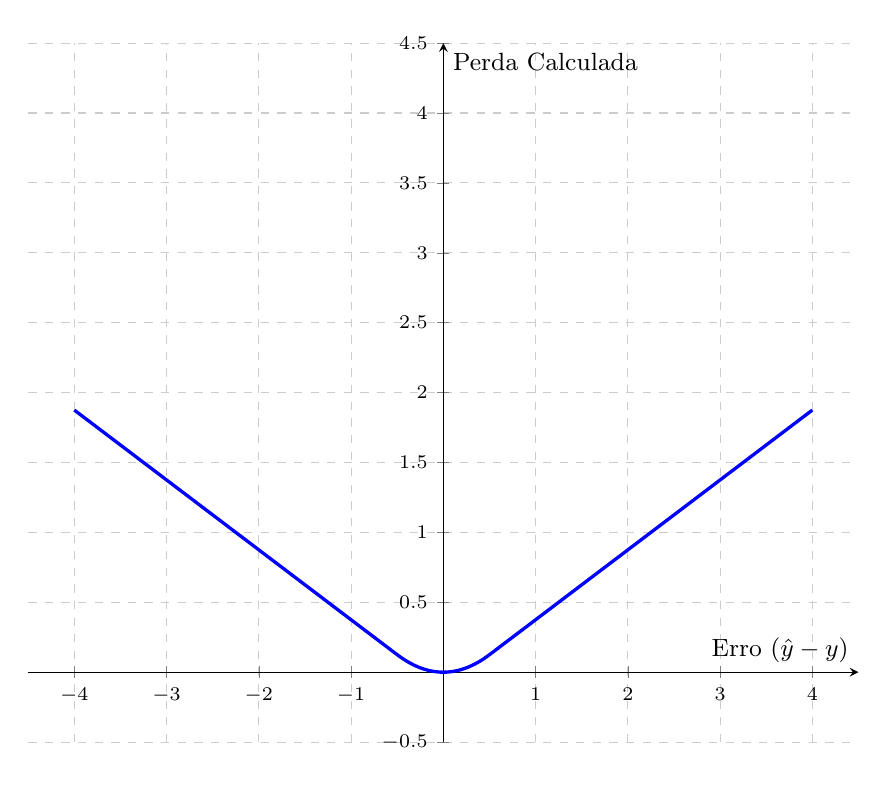
\begin{tikzpicture}
            \def\delta{0.5} % Delta pequeno
            \begin{axis}[
                xlabel={Erro ($\hat{y} - y$)},
                ylabel={Perda Calculada},
                axis lines=middle,
                grid=major,
                grid style={dashed, gray!40},
                xmin=-4.5, xmax=4.5,
                ymin=-0.5, ymax=4.5,
                legend pos=north west,
                width=\textwidth,
                label style={font=\small},
                tick label style={font=\scriptsize},
                title style={font=\bfseries, yshift=-5pt},
            ]
                % Função Huber Loss
                \addplot[
                    domain=-4:4, 
                    samples=201, 
                    color=blue, 
                    very thick,
                ] {(abs(x) <= \delta) ? (0.5*x^2) : (\delta*(abs(x) - 0.5*\delta))};
            \end{axis}
        \end{tikzpicture}
        \caption{Perda Huber com $\delta = 0.5$.}
        \label{fig:huber-comparacoes-mae}
    \end{subfigure}
    \hfill % Espaço entre as figuras
    % Figura da Direita (Parecida com MSE)
    \begin{subfigure}[b]{0.48\textwidth}
        \centering
        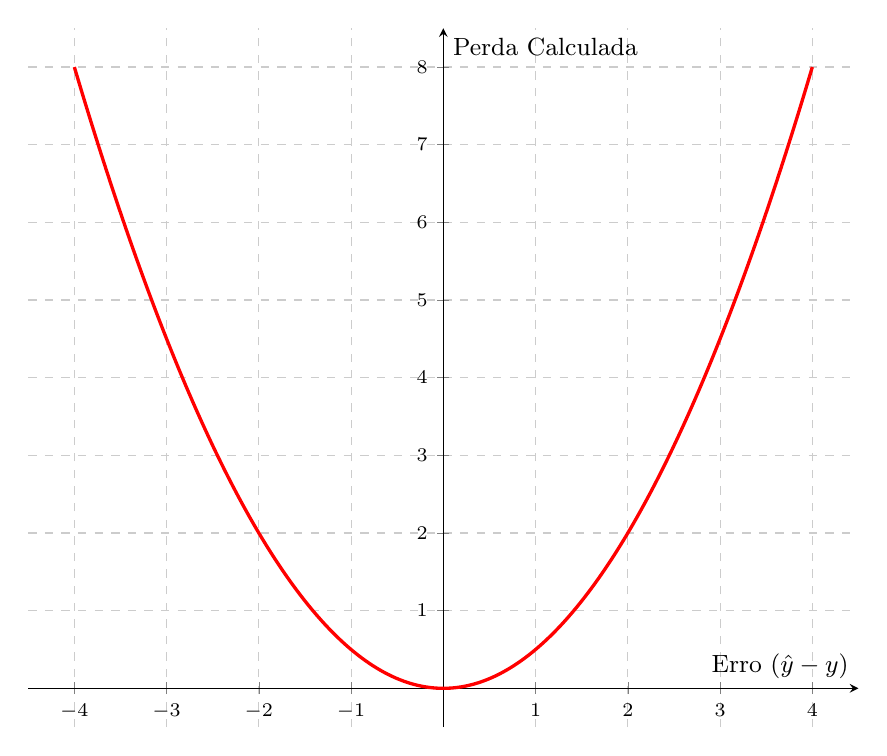
\begin{tikzpicture}
            \def\delta{4.0} % Delta grande
            \begin{axis}[
                xlabel={Erro ($\hat{y} - y$)},
                ylabel={Perda Calculada},
                axis lines=middle,
                grid=major,
                grid style={dashed, gray!40},
                xmin=-4.5, xmax=4.5,
                ymin=-0.5, ymax=8.5,
                legend pos=north west,
                width=\textwidth,
                label style={font=\small},
                tick label style={font=\scriptsize},
                title style={font=\bfseries, yshift=-5pt},
            ]
                % Função Huber Loss
                \addplot[
                    domain=-4:4, 
                    samples=201, 
                    color=red, 
                    very thick
                ] {(abs(x) <= \delta) ? (0.5*x^2) : (\delta*(abs(x) - 0.5*\delta))};

            \end{axis}
        \end{tikzpicture}
        \caption{Perda Huber com $\delta = 4.0$.}
        \label{fig:huber-comparacoes-mse}
    \end{subfigure}
    
    \caption{Comparação da Perda de Huber com diferentes valores de $\delta$.}
    \label{fig:huber-delta-comparacoes}
    \fonte{O autor (2025).}
\end{figure}

Assim, nota-se que ao utilizar a perda de Huber em um problema de regressão, é nítido que o grau de complexidade do problema pode aumentar, pois haverá mais um hiperparâmetro para ser otimizado de forma manual. Isso pode não ser ideal para cenários em que já existem muitos hiperparâmetros. Para isso, \textcite{LossesArticle} explicam que essa função é comumumente utilizada em problemas de gressão robusta, como em regressões lineares e em \textit{time series forecasting}, em que \textit{outliers} e ruído podem estar presentes.

\subsection{Perda Log-Cosh}

\section{Lidando com a Escala: Foco no Erro Relativo}

\subsection{Erro Quadrático Médio Logarítmico (MSLE)}

\section{Mudando o Objetivo da Previsão: Além da Média}

\subsection{Perda Quantílica}

\subsection{Perda Epsilon-Insensível}

\section{Perdas Baseadas em Distribuições de Dados}

\subsection{Perda de Poisson}

\subsection{Perda de Tweedie}

\subsection{Divergência Kullback-Leibler}

\section{Comparativo: Funções de Perda para Regressão}

\section{Fluxograma: Escolhendo a Função de Perda Ideal}